\documentclass[a4paper,12pt]{article}
\usepackage[margin=1in]{geometry}

\usepackage[T2A]{fontenc}			% кодировка
\usepackage[utf8]{inputenc}			% кодировка исходного текста
\usepackage[english,russian]{babel}	% локализация и переносы
\usepackage{graphicx}                % Математика
\usepackage{mathtext}
\usepackage[T2A]{fontenc}
\usepackage[utf8]{inputenc}
\usepackage{amsmath,amsfonts,amssymb,amsthm,mathtools, mathrsfs}
\usepackage{wasysym}

%Заговолок
\author{Бичина Марина 
группа Б04-005 1 курса ФЭФМ}
\title{}
\date{}


\begin{document} % начало документа

\begin{center}
\begin{Large}
{ Марина Б04-005, Лабораторная работа №3.3.4 "Эффект Холла в полупроводниках".}
\end{Large}
\end{center}
\paragraph{Цель работы:} 
\begin{enumerate}
\itemsep0em
\item исследовать зависимость ЭДС Холла от величины магнитного поля при различных значениях тока через образец для определения константы Холла 
\item определить знак носителей заряда и проводимость материала образца
\end{enumerate}
\paragraph{Оборудование:}
\begin{enumerate}
\itemsep0em
\item электромагнит с источником питания
\item амперметр
\item миллиамперметр
\item реостат
\item милливеберметр
\item цифровой вольтметр
\item источник питания (1.5 В)
\item образцы легированного германия
\end{enumerate}
\paragraph{Формулы, необходимые для расчетов:}
\paragraph{}
Эффект Холла - явление возникновения поперечной разности потенциалов при помещении проводника с постоянным током в магнитное поле.
	\begin{itemize}
		\item
			ЭДС Холла:
			\begin{equation}
				\label{E}
				U_{\perp} = U_{34} - U_0;
			\end{equation}
		\item
			Постоянная Холла:
			\begin{equation}
				\label{R}
				R_\text{н} = -\frac{U_{\perp}}{B} \cdot \frac{a}{I};
			\end{equation}
			\item
			Индукция:
			\begin{equation}
			B = \frac{\Delta \Phi}{SN}
			\end{equation}
		\item
			Концентрация носителей тока в образце:
			\begin{equation}
				\label{n}
				n = \frac{1}{R_\text{н} e}
			\end{equation}
		\item
			Удельная проводимость материала образца:
			\begin{equation}
				\label{sigma}
				\sigma = \frac{I L_{35}}{U_{35}al}
			\end{equation}
		\item
			Подвижность носителей тока:
			\begin{equation}
				\label{b}
				\mu = \frac{\sigma}{en}
			\end{equation}
		\item
			Метод наименьших квадратов $ y = a + bx $
\begin{equation}
b = \frac{\langle xy \rangle - \langle x \rangle \langle y \rangle}{\langle x^2 \rangle - \langle x \rangle^2} \;\;
a = \langle y \rangle - b \cdot \langle x \rangle
		\end{equation}
	\end{itemize}


\paragraph{Описание установки:}
\paragraph{}
Установка представлена на рисунке:

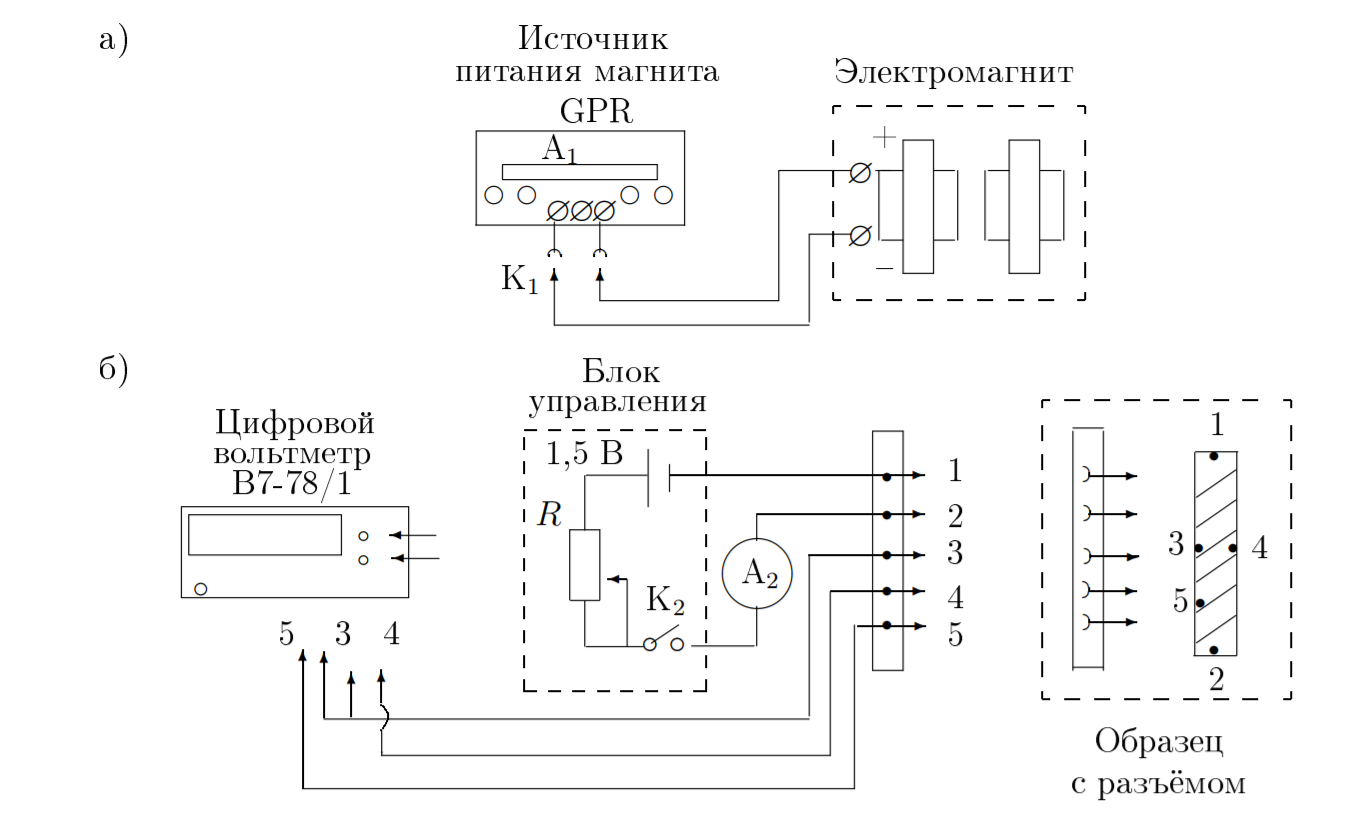
\includegraphics[scale=0.55]{Holl2.png}

В зазоре электромагнита создается (1а) создается постоянное магнитное поле, величину которого можно менять с помощью регулятора источника питания электромагнита. Ток питания электромагнита измеряется амперметром $A_1$. 

Прямоугольный образец из легированного германия, смонтированный в специальном держателе (1б) подключается к источнику питания. Величина тока регулируется реостатом $R_2$ и измеряется миллиамперметром $A_2$.

 В образце, помещенном в зазор электромагнита, между контактами 3 и 4 возникает разность потенциалов $U_{34}$,которая измеряется с помощью вольтметра $V$
\paragraph{}


\paragraph{Ход работы:}
\begin{enumerate}
	\begin{table}
		\label{table:const}
		\begin{tabular}{|c|c|c|c|}
			\hline
			\begin{tabular}[c]{@{}c@{}}Расстояние между\\ контактами 3 и 5\\ $L_{35}$, мм\end{tabular} & \begin{tabular}[c]{@{}c@{}}Толщина образца\\ $a$, мм\end{tabular} & \begin{tabular}[c]{@{}c@{}}Ширина образца\\ $l$, мм\end{tabular} & \begin{tabular}[c]{@{}c@{}}Постоянная катушки\\ $SN$, см$^2\cdot\,$вит.\end{tabular} \\ \hline
				6                                                                                          & 2,2                                                               & 7                                                                &                                                                 72                   \\ \hline
			\end{tabular}
	\end{table}
		

\item Откалибруем электромагнит: для этого установим связь между индукцией магнитного поля в зазоре электромагнита и током через обмотку магнита.
\begin{table}[h!]
\begin{center}
\begin{tabular}{|c||c|c|c|c|c|c|c|}
\hline 
$I_m$, А & 0.2 & 0.4 & 0.6 & 0.8 & 1.0 & 1.2 & 1.4 \\ 
\hline 
$B$, мТл & 242.7 & 404.5 & 632.3 & 801.0 & 921.1 & 1003.1 & 1028.3 \\ 
\hline 
\end{tabular}
\end{center}
\end{table}
\item На основе этих данных построим график зависимости $B(I)$. Получаем квадратичную зависимость

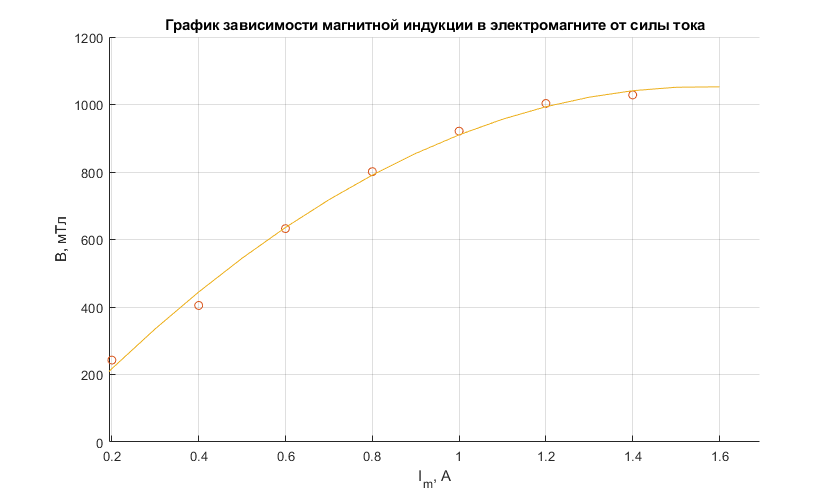
\includegraphics[scale=0.7]{kalibr.png}
\item Произведем измерения ЭДС Холла. В таблице приведены значения, при которых начальное на $U_{34}$ напряжение при $I_0=0$ уже учтено и вычтено.
\begin{table} 
\begin{center}
\begin{tabular}{|c||c|c|c|c|c|c|c|}
 \hline 
 № & 1 & 2 & 3 & 4 & 5 & 6 & 7 \\ 
 \hline 
 $I_m$, A & 0.2 & 0.4 & 0.6 & 0.8 & 1.0 & 1.2 & 1.4 \\ 
 \hline 
 \hline
 $U_{0}=66$, мкВ ($I_0=0.3$ А) & 51 & 108 & 158 & 205 & 240 & 263 & 281 \\ 
 \hline 
 $U_{0}=90$, мкВ ($I_0=0.4$ А) & 75 & 143 & 214 & 275 & 322 & 356 & 381 \\ 
 \hline 
 $U_{0} = 112$, мкВ ($I_0=0.5$ А) & 86 & 181 & 266 & 347 & 402 & 445 & 475 \\ 
 \hline 
 $U_{0} = 132$, мкВ ($I_0=0.6$ А) & 101 & 219 & 322 & 379 & 485 & 536 & 572 \\ 
 \hline 
 $U_{0} = 153$, мкВ ($I_0=0.7$ А) & 123 & 251 & 373 & 483 & 568 & 625 & 667 \\ 
 \hline 
 $U_{0} = 175$, мкВ ($I_0=0.8$А) & 140 & 293 & 429 & 552 & 648 & 715 & 762 \\ 
 \hline 
 $U_{0}=197$, мкВ ($I_0=0.9$ А) & 157 & 329 & 482 & 632 & 731 & 804 & 858 \\ 
 \hline 
 $U_{0} = 218$, мкВ ($I_0=1.0$ А) & 172 & 356 & 535 & 693 & 808 & 894 & 953 \\ 
 \hline 
 \end{tabular}
 \end{center}
 \end{table}  
 
 Далее, исходя из полученных данных, построим график зависимости $U(B)$, воспользовавшись методом наименьших квадратов (МНК). 
 
 Определим коэффициенты наклона графика $k = \dfrac{dU_{\perp}}{dB}$. 
 
 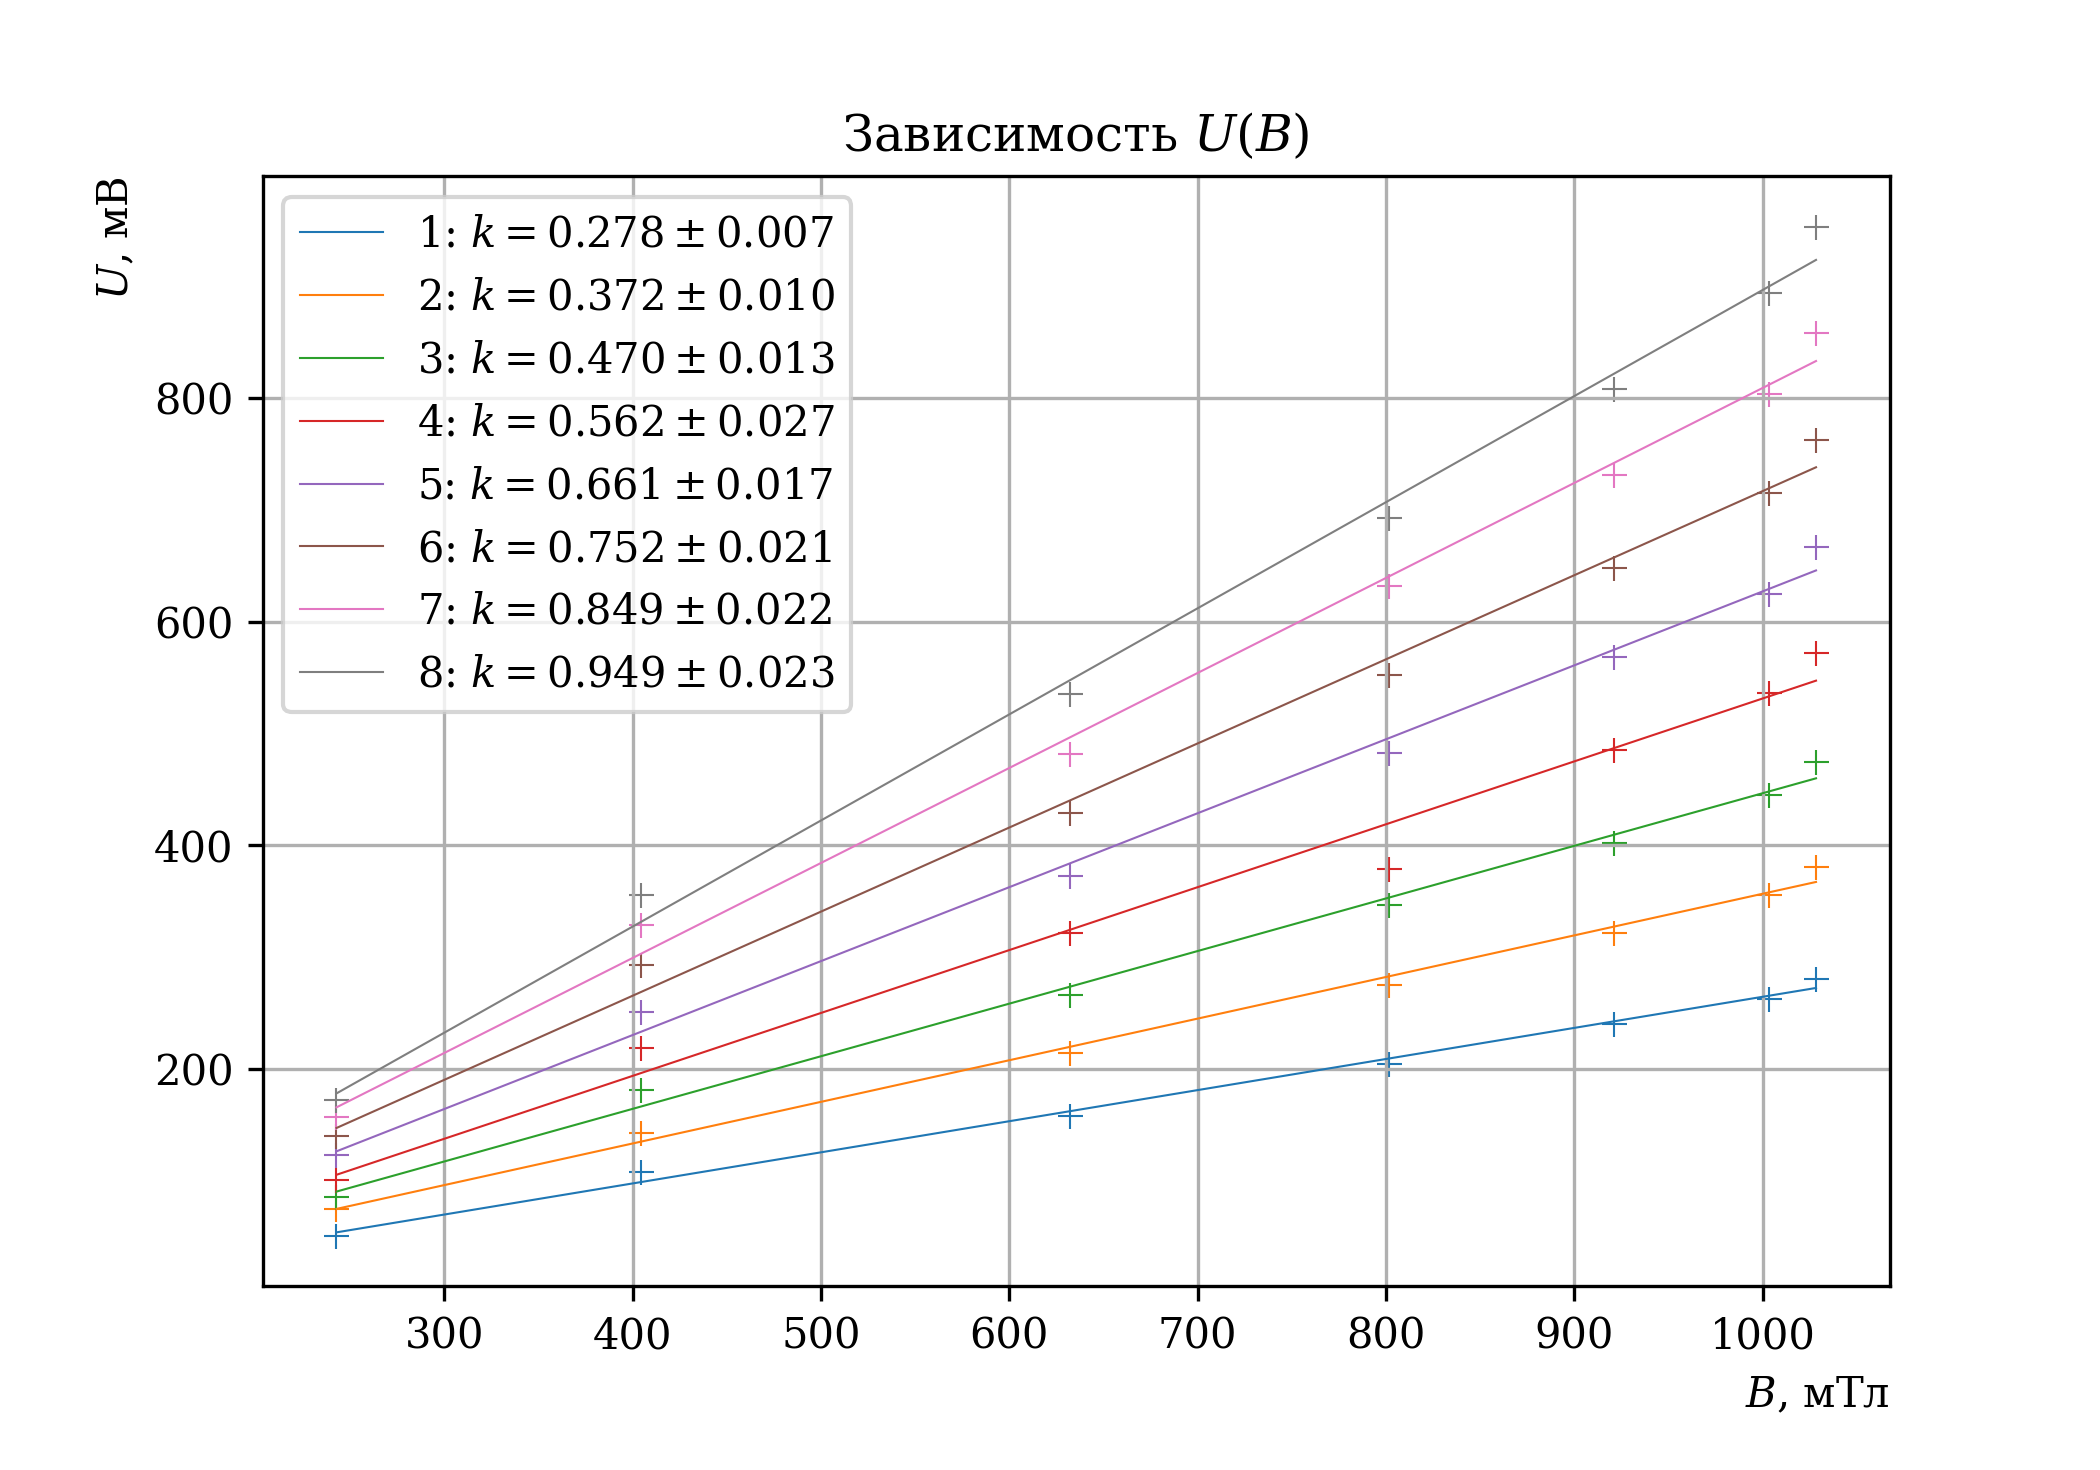
\includegraphics[scale=0.9]{plot1.png}
 
	По полученным значениям коэффициента $k$, построим график $k(I)$, пользуясь МНК. Новая переменная $k = \dfrac{dU^2_{\perp}}{dBdI}\dfrac{\text{В}}{\text{Тл}\cdot \text{А}}$
 
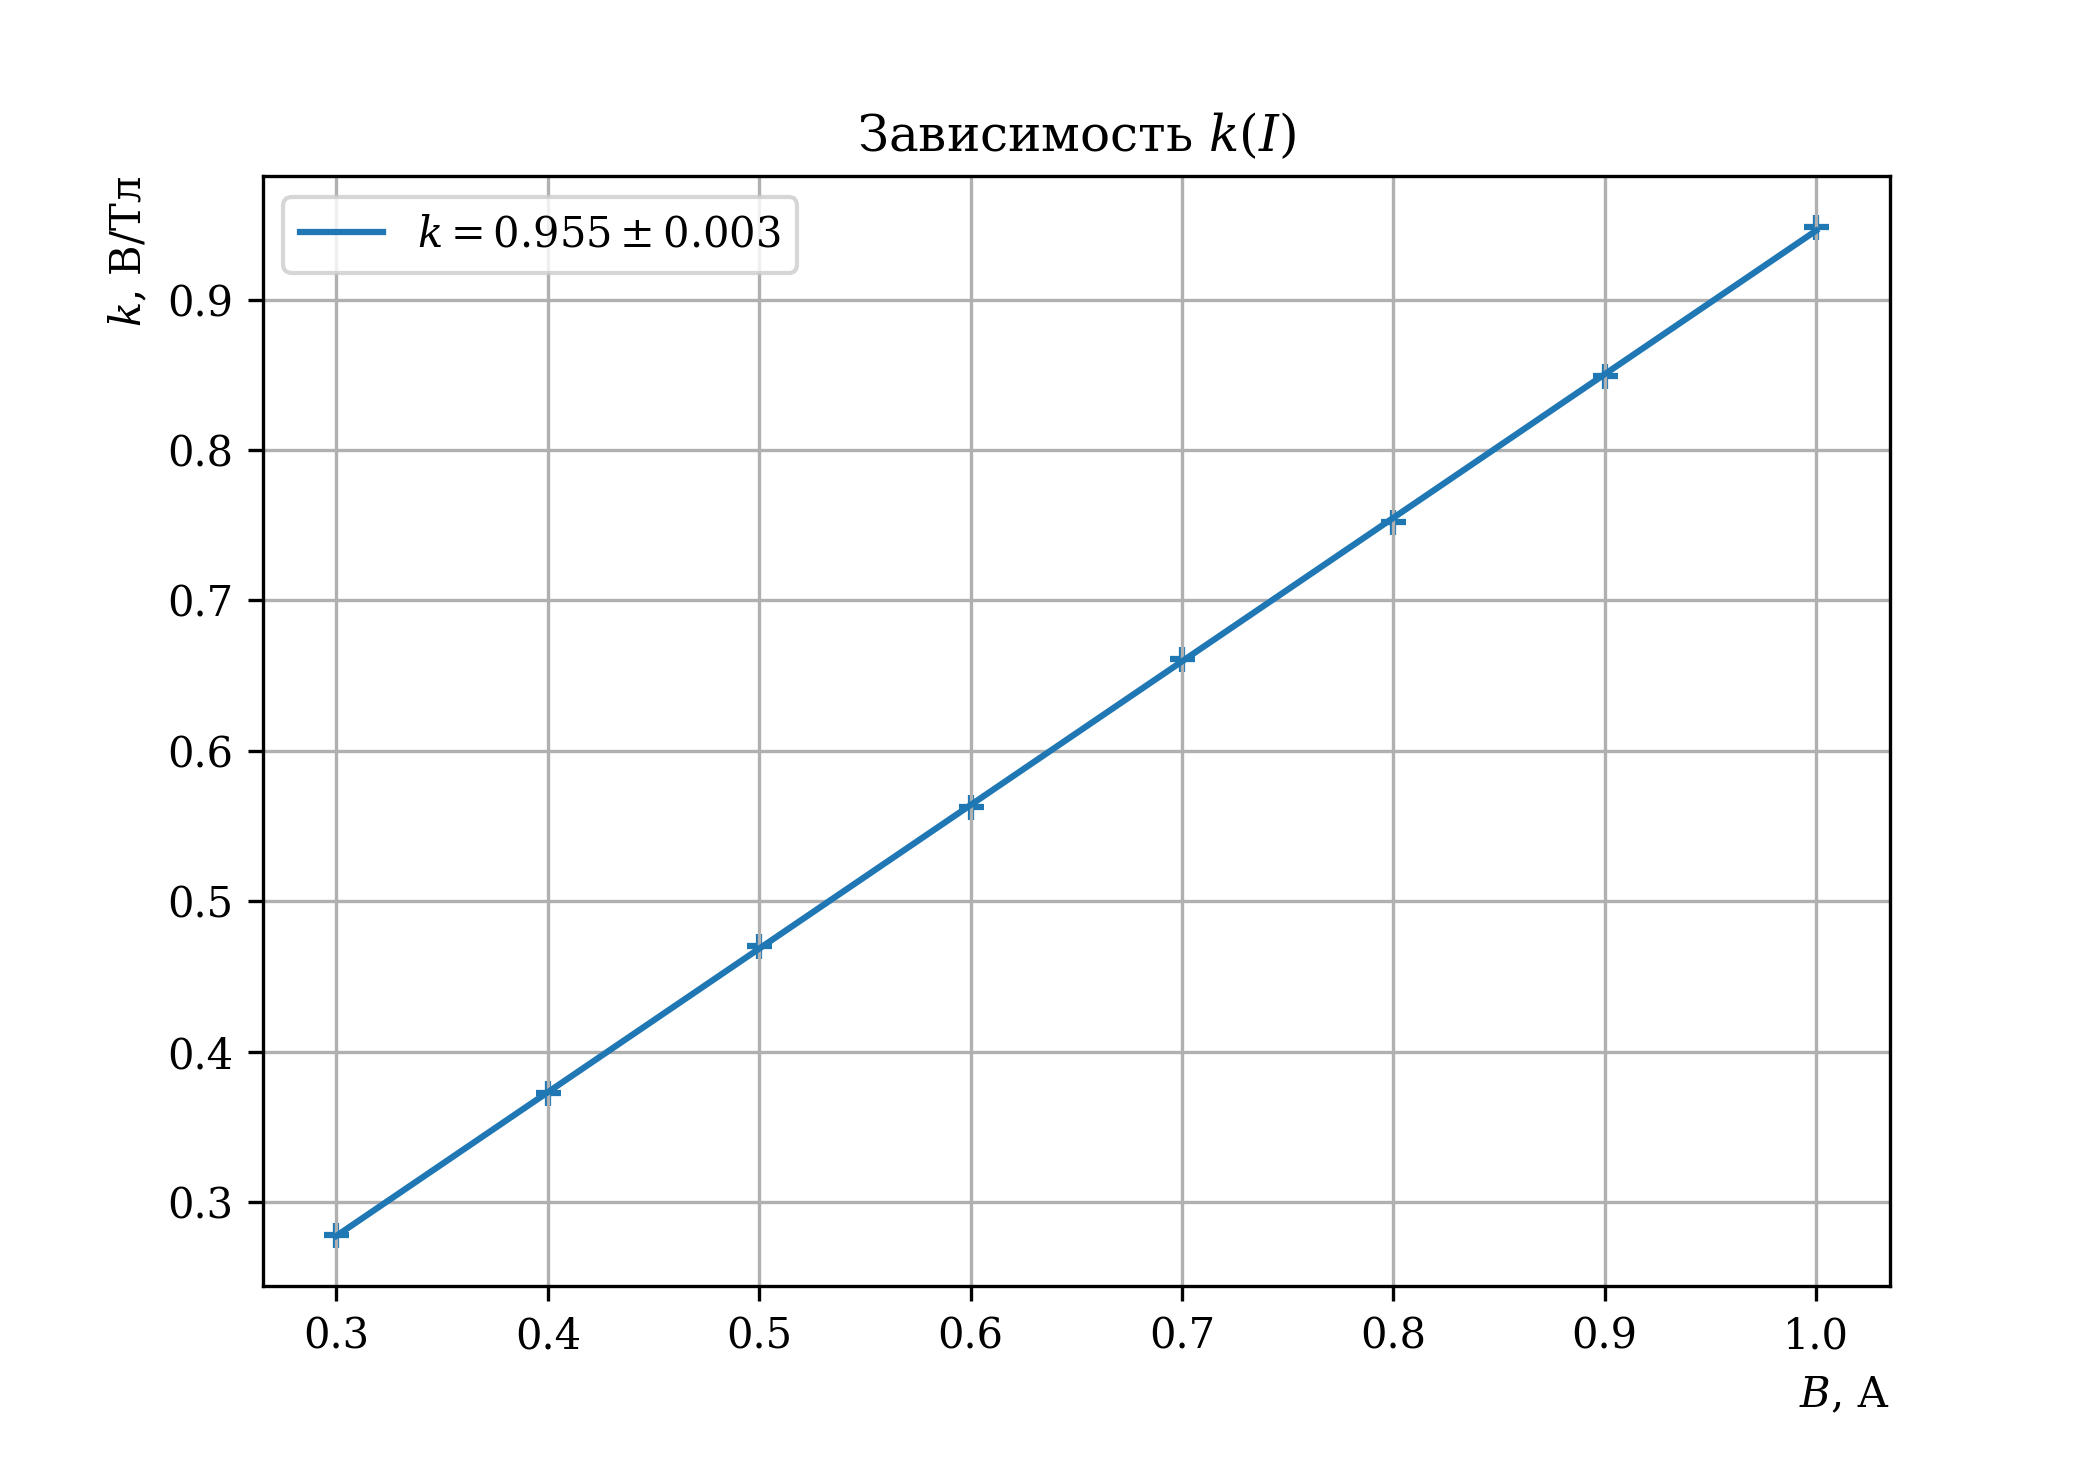
\includegraphics[scale=0.9]{plot2.png}

	
$k \cdot h = 0.96 \cdot 0.22 = 0.21\;\;\dfrac{\text{В} \cdot \text{см}}{\text{Тл} \cdot \text{А}}$

\item  По формуле (2) рассчитаем постоянную Холла по:
\begin{equation*}
R_{\text{н}} = 0.96 \cdot 72 = 691.2\;\;\frac{\text{см}^3}{\text{Кл}}
\end{equation*}

\item  По формуле (4) рассчитаем концентрацию носителей тока:
\begin{equation*}
n = \frac{1}{691.2 \cdot 1.6 \cdot 10^{-19 }} = 9.04 \cdot 10^{15}\;\; \text{см}^3
\end{equation*}
\item Измерим $U_{35} = 4,07$ мВ
 По формуле (5) рассчитаем удельную проводимость:
\begin{equation*}
\sigma = \frac{ 5 \cdot 10^{-7}}{4.07 \cdot 0.22 \cdot 7} = 1.38\;\; ( \text{Ом} \cdot \text{cм})^{-1}
\end{equation*}
Найдем подвижность электронов по формуле (6):
\begin{equation*}
\mu = \frac{1.38}{9.04 \cdot 10^{15} \cdot 1.6 \cdot 10^{-19}} = 954\;\; \frac{\text{см}^2}{B \cdot \text{c}}
\end{equation*}
\end{enumerate}
\paragraph{Выводы:}
\begin{enumerate}
\item Установили линейную зависимость ЭДС Холла от величины магнитного поля при различных значениях тока через образец 
\item Рассчитали значения постоянной Холла $R_{\text{н}} = 691.2\;\;\dfrac{\text{см}^3}{\text{Кл}}$ \\\\
Подвижность электронов $\mu = = 954\;\; \dfrac{\text{см}^2}{B \cdot \text{c}}$
\item Обнаружили дырочную зависимость 
\end{enumerate}
\end{document}